\documentclass[10pt]{beamer}

\usetheme{metropolis}
\usepackage{appendixnumberbeamer}

\usepackage{booktabs}
\usepackage[scale=2]{ccicons}
\usepackage{graphicx}
\usepackage{hyperref}
\usepackage{circuitikz}
\usepackage{pdflscape}
\usepackage{smartdiagram}

\usepackage{color}
\usepackage{listings}

\lstset{
	basicstyle=\footnotesize\ttfamily,
    keepspaces=true,
    showstringspaces=false,
    language=PHP,
    commentstyle=\ttfamily,
}

\usepackage[OT4]{polski}
\usepackage[utf8]{inputenc}

\usepackage{pgfplots}
\usepgfplotslibrary{dateplot}

\usepackage{xspace}
\newcommand{\themename}{\textbf{\textsc{metropolis}}\xspace}

\setbeamertemplate{frame footer}{}
\setbeamertemplate{frame numbering}{}

\usetikzlibrary{shapes,arrows}

\tikzstyle{decision} = [diamond, draw, fill=blue!20, 
    text width=4.5em, text badly centered, node distance=3cm, inner sep=0pt]
\tikzstyle{block} = [rectangle, draw, fill=blue!20, 
    text width=5em, text centered, rounded corners, minimum height=4em]
\tikzstyle{line} = [draw, -latex']
\tikzstyle{cloud} = [draw, ellipse,fill=red!20, node distance=3cm,
    minimum height=2em]


\title{Narzędzia deweloperskie}

\subtitle{Projektowanie i programowanie systemów internetowych I}
\author{mgr inż. Krzysztof Rewak}
\date{\today}
\institute{Wydział Nauk Technicznych i Ekonomicznych \\ Państwowa Wyższa Szkoła Zawodowa im. Witelona w Legnicy}

\begin{document}

\maketitle

\begin{frame}{Plan prezentacji}
  \setbeamertemplate{section in toc}[sections numbered]
  \tableofcontents[hideallsubsections]
\end{frame}


\section{Edytor czy IDE?}

\begin{frame}{Wprowadzenie}
	Kod musi zostać jakoś zapisany.

	Z grubsza można wyodrębnić trzy sposoby na zapisywanie kodu:
	\begin{itemize}
		\item CLI
		\item edytory tekstu
		\item IDE
	\end{itemize}
\end{frame}

\begin{frame}{CLI}
	CLI (ang. \emph{Command Line Interface}), czyli interfejs wiersza poleceń, to najbardziej podstawowy sposób interakcji człowieka z maszyną.
	
	Jest dostępny na systemach UNIX-owych (kolejne dystrybucje linuksa, macOS) oraz Windowsie:
	\begin{itemize}
		\item sh, csh, \textbf{zsh}
		\item Terminal
		\item cmd.exe, Windows PowerShell, \textbf{Cmder}
	\end{itemize}
\end{frame}

\begin{frame}{CLI}
	Z poziomu CLI można nie tylko wydawać polecenia, ale również edytować pliki z kodem. Najpopularniejsze (nie należy mylić z najlepszymi) rozwiązania to:
	\begin{itemize}
		\item vi/vim
		\item nano
		\item Emacs
		\item gedit
	\end{itemize}
	
	Istnieją miłośnicy takiego sposobu programowania, jednakże należy pamiętać, że są to rozwiązania w dużej mierze prymitywne w przypadku pracy nad poważniejszymi projektami.
\end{frame}

\begin{frame}{CLI}
	\begin{figure}[t]
		\centering
		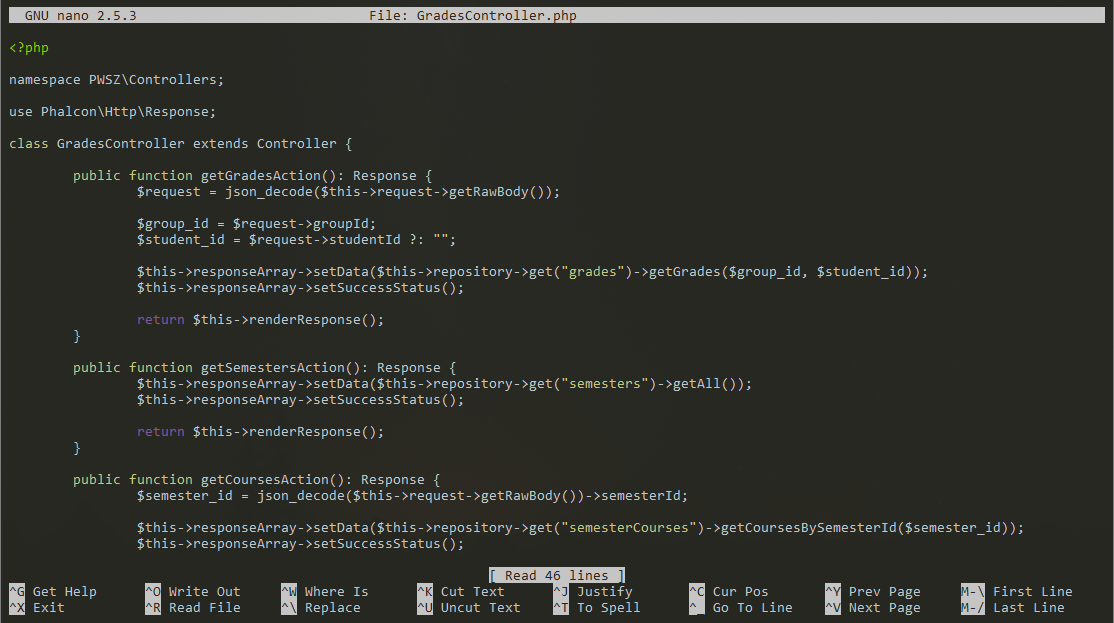
\includegraphics[width=\linewidth]{cmder.png}
		\caption{Windowsowy shell Cmder z uruchomionym nano na linuksie}
	\end{figure}
\end{frame}

\begin{frame}{Edytory tekstu}
	Programiści bardzo często używają edytorów tekstu - często równocześnie z pracą z IDE. Cechuje jest szybkość działania, możliwość pracy na dużych plikach, wiele kombinacji klawiszowych ułatwiających pracę oraz możliwość rozszerzania przez dodatki lub wtyczki.
\end{frame}

\begin{frame}{Edytory tekstu}
	Kiedy edytor tekstu wystarczy?
	\begin{itemize}
		\item przy projektach w językach ze słabym lub dynamicznym typowaniem, gdzie IDE często nie spełnia stuprocentowo swojej roli
		\item przy mniejszych projektach
		\item jeżeli programista nie potrzebuje ,,magii'' IDE
	\end{itemize}
\end{frame}

\begin{frame}{Edytory tekstu}
	Popularne edytory tekstu:
	\begin{itemize}
		\item Notepad++
		\item \textbf{Sublime Text 3}
		\item Atom
		\item Visual Studio Code
	\end{itemize}
	
	Warto zapoznać się z listami najpopularniejszych rozszerzeń do wybranego edytora, a także nauczyć się najpotrzebniejszych skrótów klawiszowych.
\end{frame}

\begin{frame}{Edytory tekstu}
	\begin{figure}[t]
		\centering
		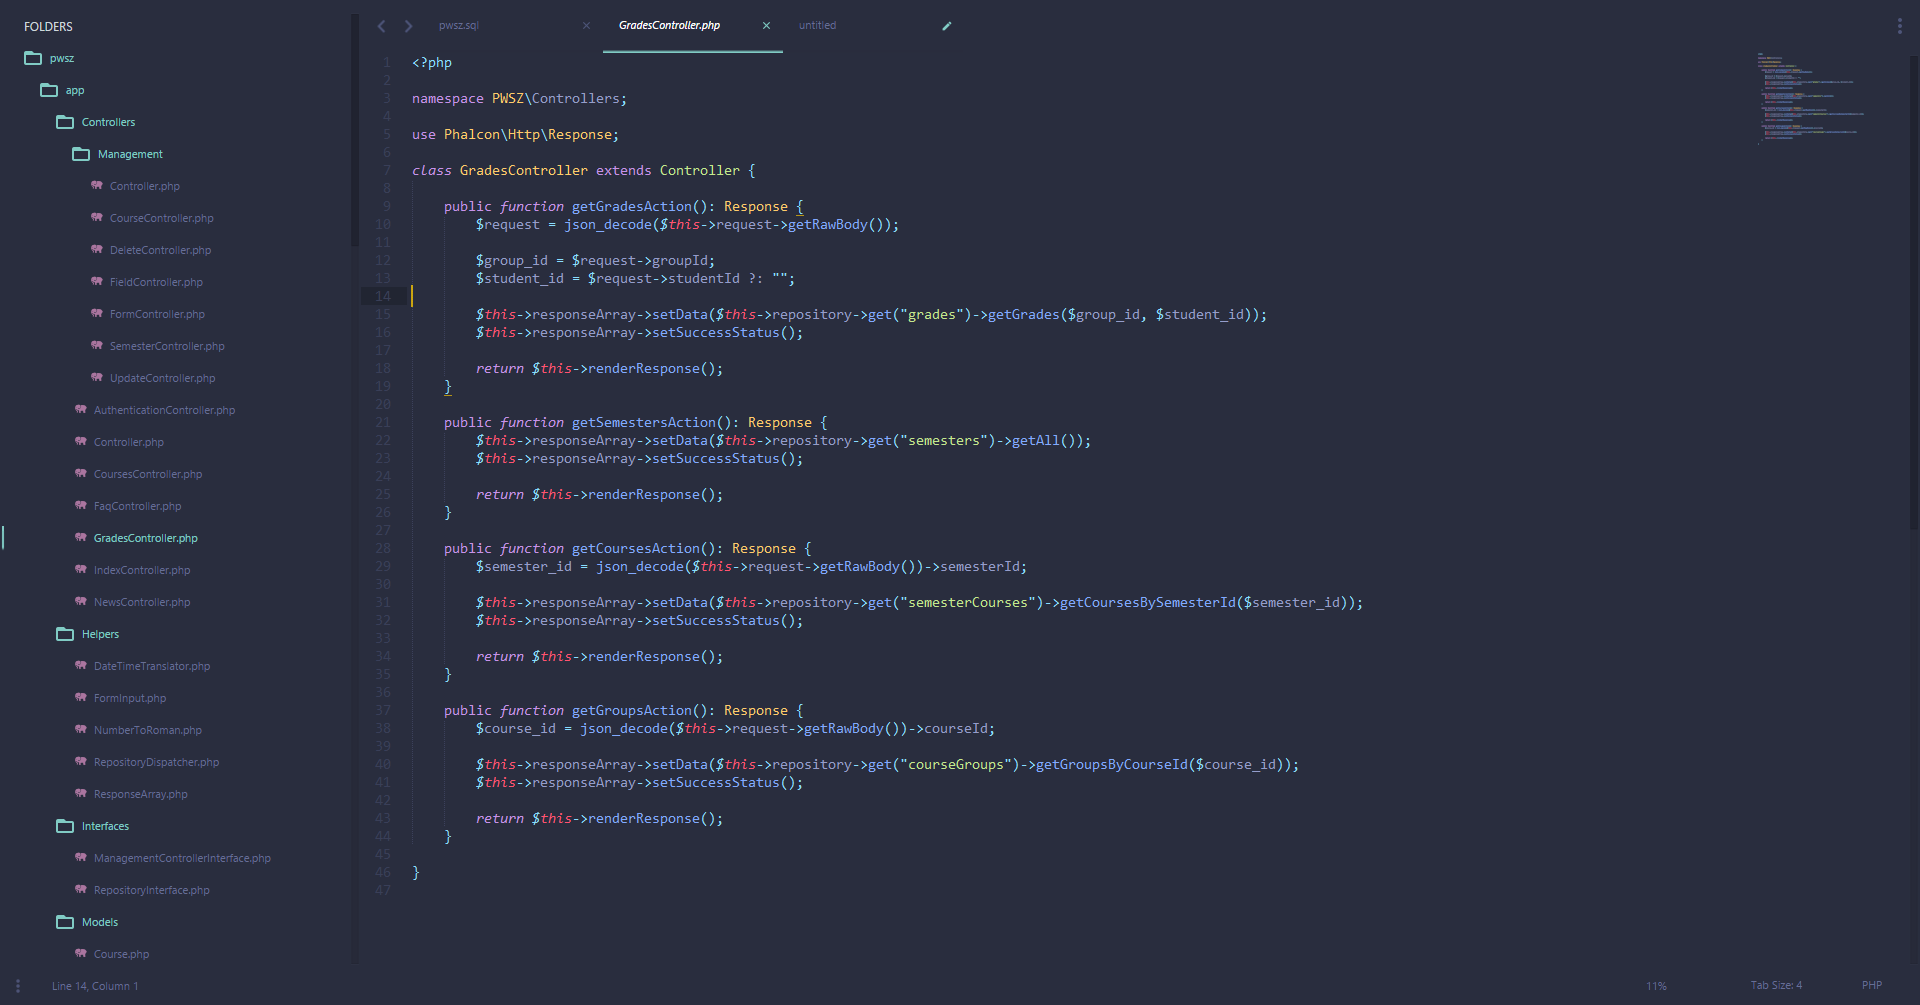
\includegraphics[width=\linewidth]{sublime.png}
		\caption{Sublime Text 3}
	\end{figure}
\end{frame}

\begin{frame}{No to IDE}
	\emph{Integrated development environment}, czyli \textbf{zintegrowane środowisko programistyczne}, to specjalistyczne oprogramowanie służące do tworzenia oprogramowania.
\end{frame}

\begin{frame}{IDE}
	Niektóre zalety i wady korzystania z IDE:
	\begin{itemize}
		\item + wszystkie narzędzia w jednym miejscu
		\item + interpretacja kodu
		\item + pełna możliwość konfiguracji
		\item - zazwyczaj kosztowne
		\item - obciążające komputer
		\item - niektórzy powiedzą, że rozleniwiające
	\end{itemize}
\end{frame}

\begin{frame}{IDE}
	Przykładowe i popularne IDE:
	\begin{itemize}
		\item Microsoft Visual Studio (C\#, C++, VB i inne)
		\item Eclipse (przede wszystkim Java)
		\item NetBeans (Java)
		\item Code::Blocks (C, C++)
		\item rozwiązania JetBrains:
		
		\begin{itemize}
			\item PhpStorm (PHP)
			\item PyCharm (Python)
			\item IntelliJ IDA (Java)
			\item WebStorm (JavaScript)
			\item CLion (C, C++)
			\item RubyMine (Ruby)
		\end{itemize}
	\end{itemize}
\end{frame}

\begin{frame}{IDE}
	\begin{figure}[t]
		\centering
		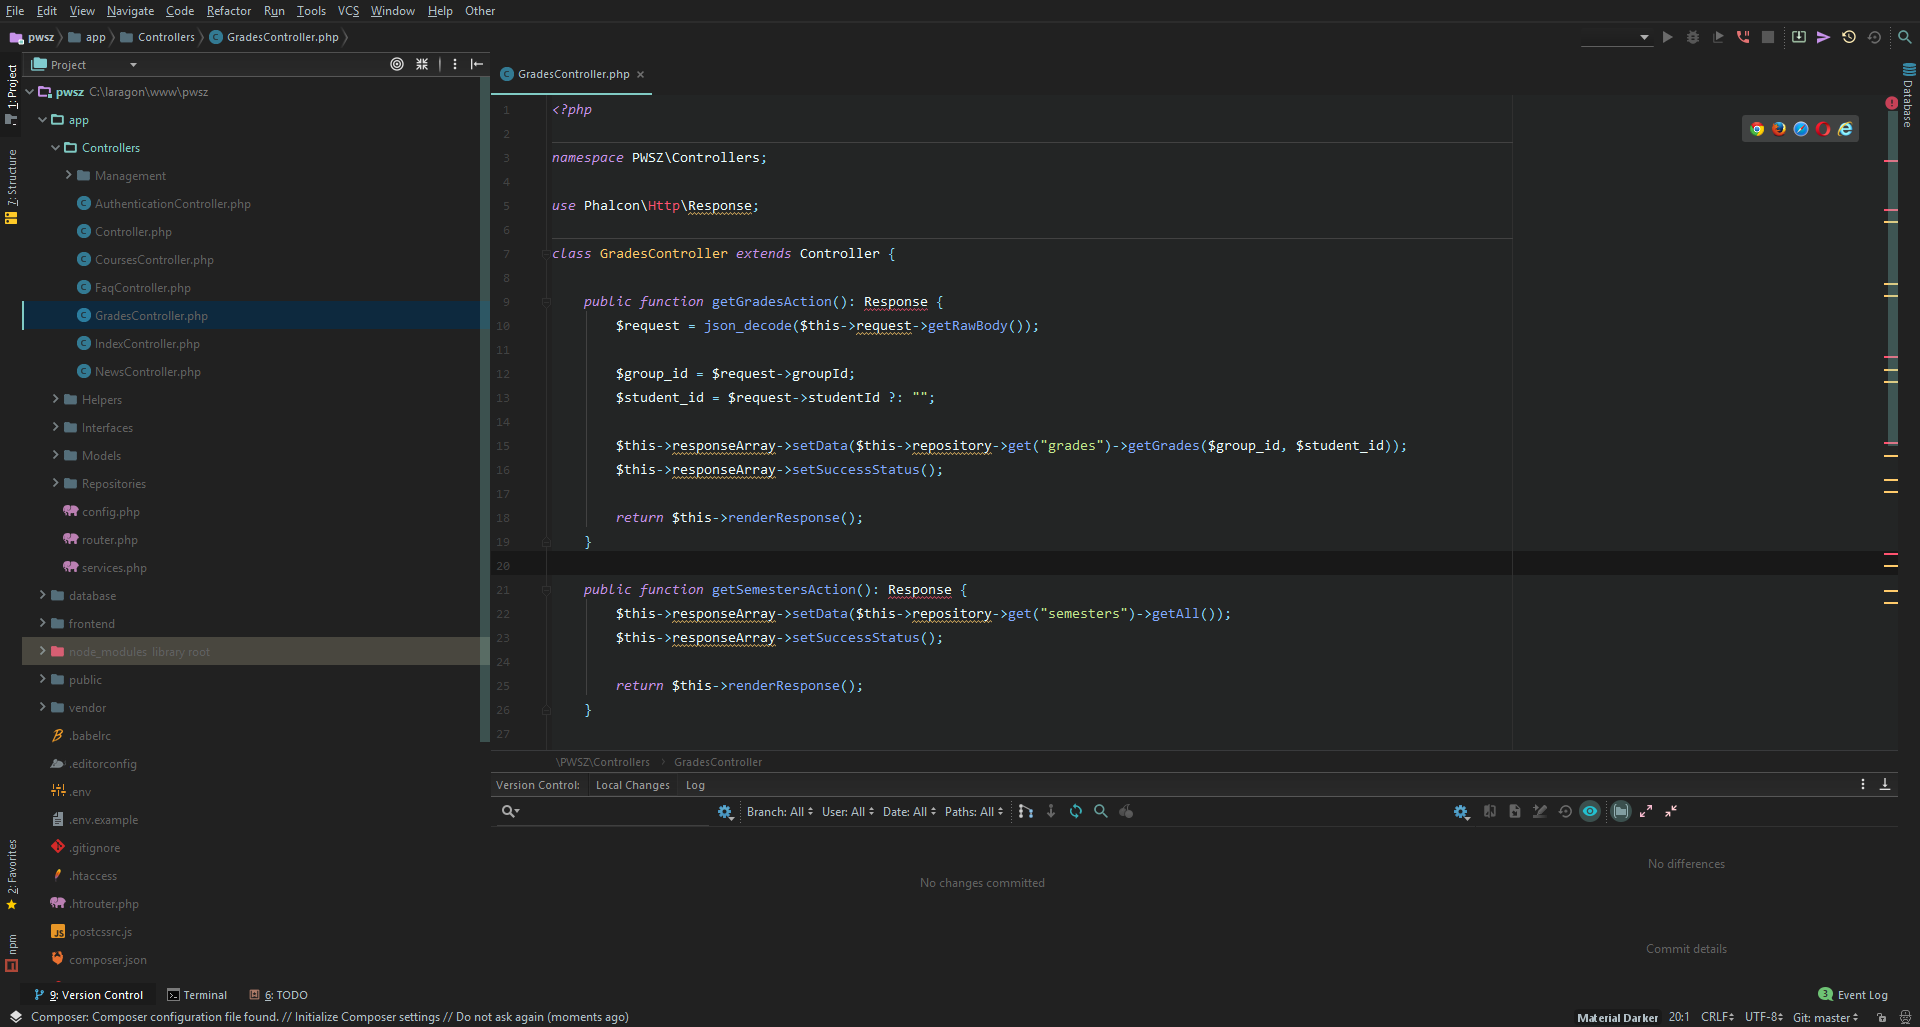
\includegraphics[width=\linewidth]{phpstorm.png}
		\caption{PhpStorm}
	\end{figure}
\end{frame}

\section{Przeglądarki internetowe}

\begin{frame}{Przeglądarki internetowe}
	\textbf{Przeglądarka internetowa} to program pozwalający przede wszystkim na wyświetlanie stron internetowych. Współczesne przeglądarki oczywiście oferują wiele innych funkcji, jednak nas będą interesowały tylko te, które mogą być przydatne dla programisty.
\end{frame}

\begin{frame}{Przeglądarki internetowe}	
	Najpopularniejsze obecnie przeglądarki internetowe:	
	\begin{itemize}
		\item Google Chrome
		\item Mozilla Firefox
		\item Internet Explorer
		\item Edge
		\item Safari
		\item Opera
	\end{itemize}
\end{frame}

\begin{frame}{Przeglądarki internetowe}	
	Przeglądarki internetowe oferują najczęściej dwa podstawowe narzędzia dla programistów.
\end{frame}

\begin{frame}{Przeglądarki internetowe}		
	Pierwszym jest prymitywne wyświetlenie źródła strony i zazwyczaj można je wywołać kombinacją klawiszy Ctrl+U. Źródło strony to nic innego jak przedstawienie w formie kodu HTML-a, który buduje daną stronę.
\end{frame}

\begin{frame}{Przeglądarki internetowe}	
	Drugi to narzędzia deweloperskie (najczęściej pod F12) i do nich możemy zaliczyć m. in. inspektora drzewa DOM, konsolę JavaScript, debuger, edytor stylów, podgląd połączeń w sieci czy narzędzia statystyczne.
\end{frame}

\begin{frame}{Przeglądarki internetowe}
	\begin{figure}[t]
		\centering
		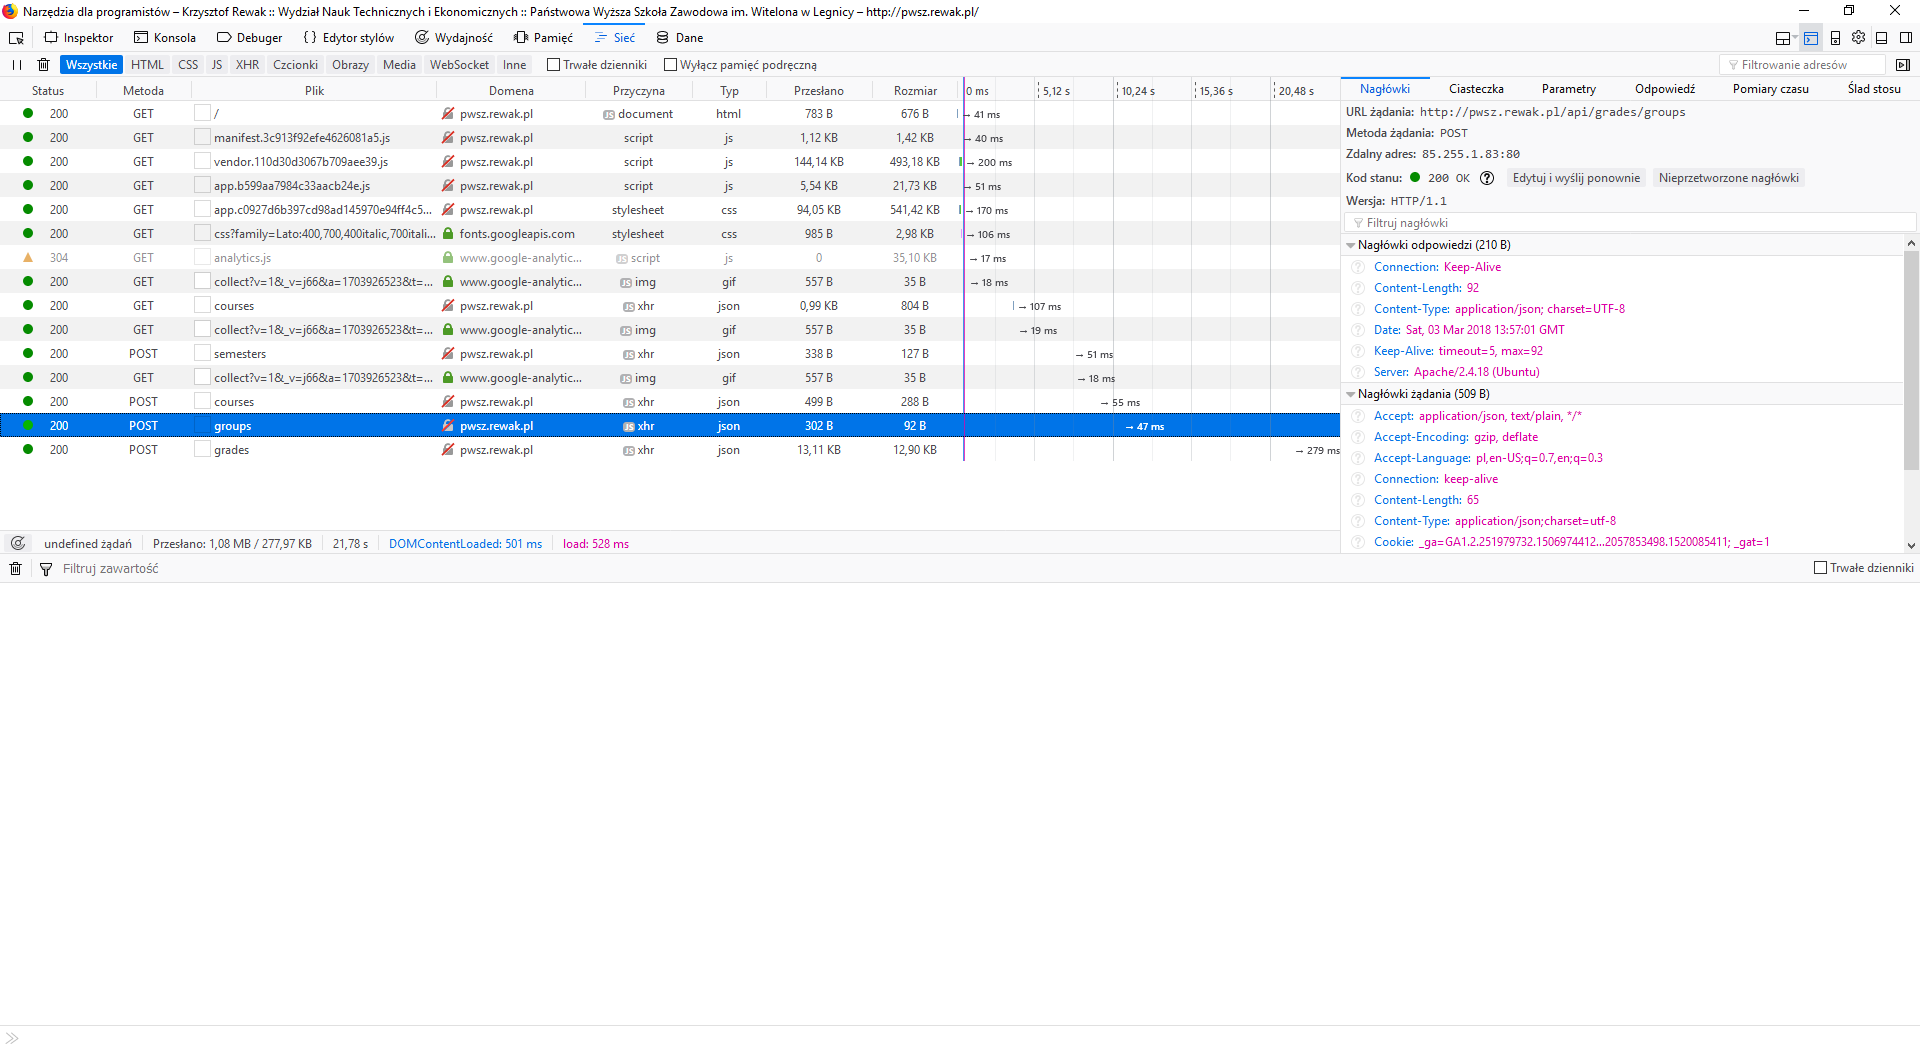
\includegraphics[width=\linewidth]{firefox.png}
		\caption{Narzędzia deweloperskie w Firefoksie}
	\end{figure}
\end{frame}

\begin{frame}{Przeglądarki internetowe}
	\begin{figure}[t]
		\centering
		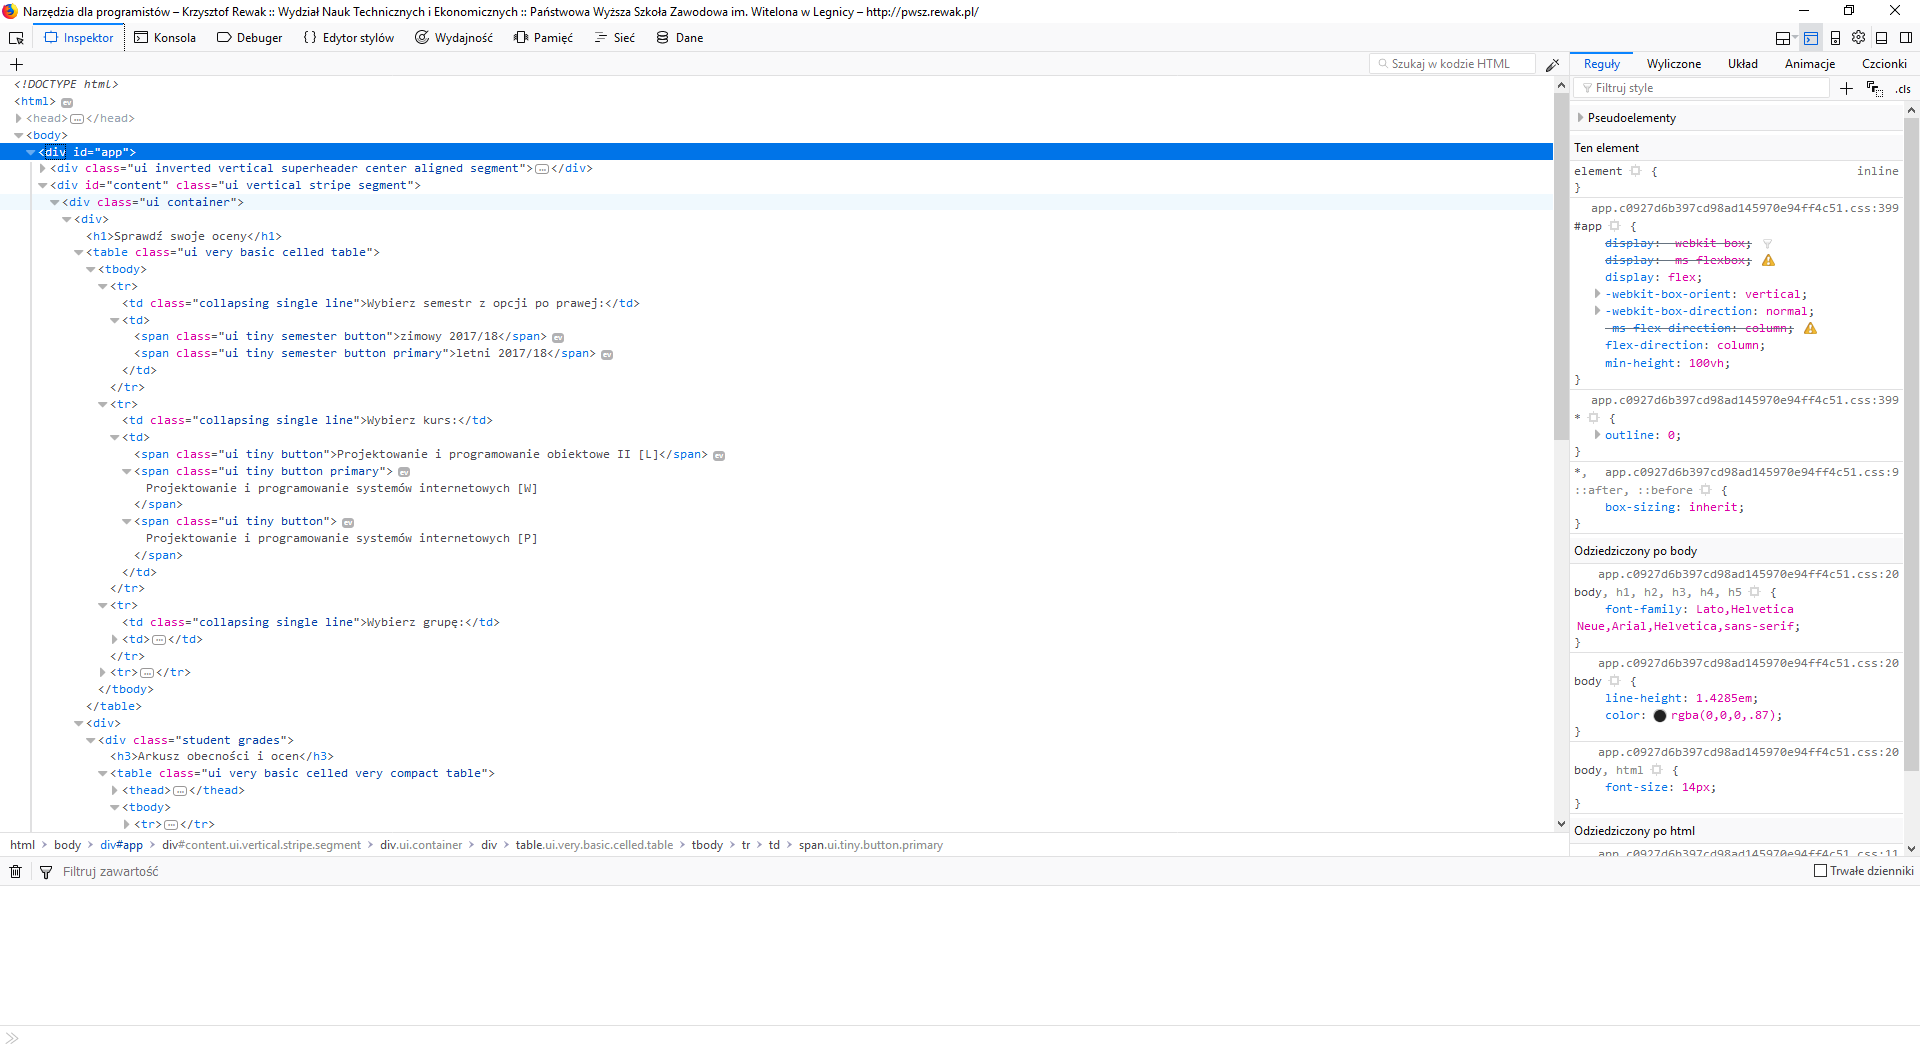
\includegraphics[width=\linewidth]{firefox2.png}
		\caption{Inspektor w Firefoksie}
	\end{figure}
\end{frame}

\section{Oprogramowanie dla programisty}

\begin{frame}{Środowiska programistyczne}
	Wygodną sprawą są predefiniowane środowiska programistyczne, które są zebranymi najpotrzebniejszymi serwisami, które są wymagane do tworzenia aplikacji. Wartym spróbowania jest Laragon, który oferuje następujące zestawy:
	\begin{itemize}
		\item WAMP, czyli Apache lub Nginx, PHP, MySQL, npm, git i inne
		\item ROR, czyli Ruby, Postres, npm, Redis i git
		\item MEAN, czyli Node, Mongo i git
		\item Python, Postres, Redis i git
		\item Spring, czyli Java, Maven, git
		\item Golang, czyli Go, Postgres, Redis i git
	\end{itemize}
	
	Powinno to zaspokoić potrzeby każdego początkującego programisty, a jednocześnie nie zmusi go do wielogodzinnej konfiguracji środowiska.
\end{frame}

\begin{frame}{Łączenie się z serwerem}
	Po wdrożeniu systemu internetowego na zewnętrzny serwer z pewnością zajdzie potrzeba ponownego połączenia się z aplikacją. W środowisku Windows pomogą następujące programy:
	\begin{itemize}
		\item ssh: Cmder lub PuTTY
		\item scp: WinSCP
		\item ftp: Total Commander
	\end{itemize}
\end{frame}

\begin{frame}{Podgląd baz danych}
	W przypadku pracy z systemem internetowym wykorzystującym bazy danych warto zainteresować się narzędziami przeznaczonymi do zarządzania bazami:
	\begin{itemize}
		\item HeidiSQL
		\item MySQL Workbench
		\item phpMyAdmin
	\end{itemize}
\end{frame}

\begin{frame}{Podgląd baz danych}
	\begin{figure}[t]
		\centering
		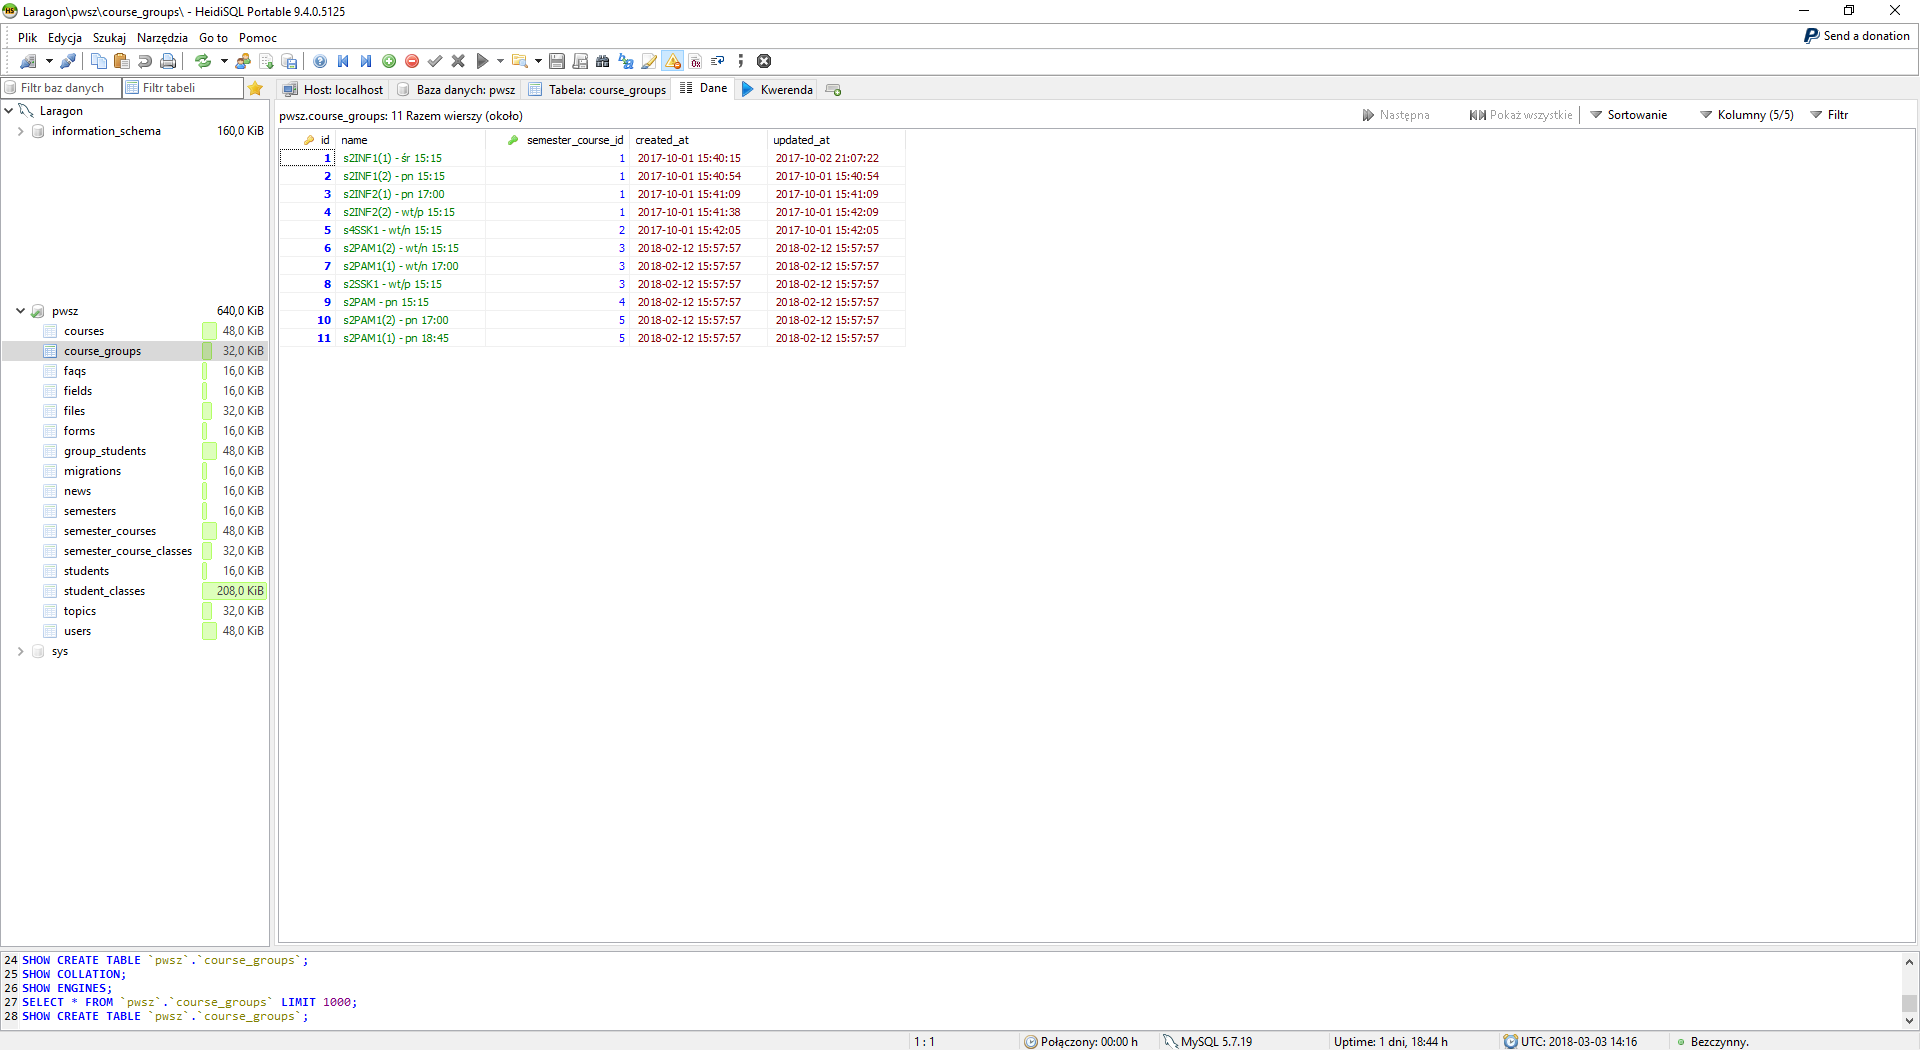
\includegraphics[width=\linewidth]{heidisql.png}
		\caption{HeidiSQL podłączona do bazy danych}
	\end{figure}
\end{frame}

\begin{frame}{Systemy zarządzania zależnościami}
	Każdy język ma własny system zarządzania zależnościami. Pomagają one w procesie deweloperskim przy dodawaniu i utrzymywaniu wersji zewnętrznych modułów, paczek, pakietów lub innych zależności.
	
	Warto wiedzieć jaki język ma jaki system:

	\begin{itemize}
		\item PHP: Composer
		\item .NET: NuGet
		\item Java: Maven
		\item JavaScript: npm
		\item Ruby: RubyGems
		\item Python: Pipenv
	\end{itemize}
\end{frame}

\begin{frame}{Git}
	Jednym z podstawowych narzędzi pracy w każdym sensownym projekcie powinien być system kontroli wersji. Obecnie najpopularniejszym jest Git, ale korzysta się również z Subversion (SVN) lub Mercuriala. Z Gita można korzystać na kilka sposobów:
	
	\begin{itemize}
		\item z poziomu CLI
		\item z poziomu IDE
		\item wykorzystując dedykowane oprogramowanie:
		\begin{itemize}
			\item Sourcetree
			\item Github Desktop
			\item GitKraken
		\end{itemize}
	\end{itemize}
\end{frame}

\begin{frame}{Wirtualizacja, konteneryzacja}
	Wielu programistów korzysta z tzw. maszyn wirtualnych. Są to odizolowane uruchomienia innych programów, a w szczególności systemów operacyjnych. Popularnym narzędziem tego typu jest \textbf{VirtualBox}.
\end{frame}

\begin{frame}{Wirtualizacja, konteneryzacja}
	Innym ciekawym rozwiązaniem jest \textbf{Vagrant}. Pozwala on na zautomatyzowanie procesu konfiguracji i ustawiania środowiska deweloperskiego. Korzysta pod spodem z rozwiązań VirtualBoksa i z poziomu skryptów konfiguracyjnych jest w stanie stworzyć dowolny zestaw narzędzi programistycznych.
\end{frame}

\begin{frame}{Wirtualizacja, konteneryzacja}	
	Jeszcze inną rzeczą jest \textbf{Docker} i konteneryzacja. Zamiast wirtualizować cały system operacyjny można tworzyć wydzielone kontenery z konkretnymi serwisami takimi jak bazy danych, interpretery języków lub inne serwisy. Takie zestaw pasujących do siebie klocków jest łatwy do przenoszenia i konfiguracji.
\end{frame}

\section{Podsumowanie}

\begin{frame}{Bibliografia i ciekawe źródła}
  
	\begin{thebibliography}{9}
	
		\bibitem{sublime}
		https://www.sublimetext.com/
		
		\bibitem{laragon}
		https://laragon.org/download/
		
		\bibitem{laragon}
		https://laragon.org/download/
	
	\end{thebibliography}

\end{frame}

\appendix

\begin{frame}[standout]
	Pytania?
\end{frame}

\begin{frame}{}

	Kod prezentacji dostępny jest w repozytorium git pod adresem \texttt{https://bitbucket.org/krewak/pwsz-ppsi} \\ \ \\

	\begin{figure}
		\centering
		\href{https://bitbucket.org/krewak/pwsz-ppsi}{
			
\includegraphics[width=.15\textwidth]{../_template/bitbucket.png}
		}
	\end{figure}
	
	Wszystkie informacje dot. kursu dostępne są pod adresem \texttt{http://pwsz.rewak.pl/kursy/4} \\ \ \\

	\begin{figure}
		\centering
		\href{http://pwsz.rewak.pl/kursy/3}{
			
\includegraphics[width=.15\textwidth]{../_template/rewak.png}
		}
	\end{figure}

\end{frame}

\end{document}
